\documentclass[11pt,a4paper,parskip=full]{scrartcl}
\usepackage[utf8]{inputenc}
\usepackage{graphicx}
\usepackage{float}
\usepackage[ngerman]{babel}
\usepackage[babel, german=quotes]{csquotes}
\usepackage[hidelinks]{hyperref}
\usepackage{amsmath}
\usepackage[
style=numeric-comp,
backend=biber,
bibencoding=utf8,
bibwarn=true,
doi=false,
url=false,
sorting=none
]{biblatex}
\addbibresource{bibliography.bib}

\author{Michael Wolz}
\title{Popularität von Java-Annotationen im zeitlichen Verlauf\\\Large{Fortgeschrittene Softwaretechnik}\\ \large{Wintersemester 2017/2018}}

\begin{document}

\maketitle

\section{Reflexion}

Die in der Vorlesung behandelte zeitliche Analyse der Entwicklung von JUnit-Testmetho\-den mithilfe von BOA weckte bereits großes Interesse bei mir. Gerade die Entwicklung von verschiedenen Veränderungen an Quellcodes über die Zeit finde ich sehr interessant und somit bot es sich an, dass ich mich im Rahmen des Abschlussprojektes für das Modul \textit{Fortgeschrittene Softwaretechnik} mit der Popularität von Java-Annotationen im zeitlichen Verlauf beschäftige. Hierbei werden zunächst die Häufigkeiten von Java-Annotationen betrachtet und anschließend die meist verwendeten Annotationen im zeitlichen Verlauf analysiert. Die für die Analyse herangezogenen Daten stammen dabei aus dem GitHub September 2015 Datensatz von BOA, welcher insgesamt 380125 Repositories beinhaltet \cite{boadatasetstats}. Die Daten werden im Anschluss mit R verarbeitet und ausgewertet.

\section{Datenbeschaffung mit BOA}

Im Ordner \texttt{boa} befindet sich das Skript, welches zur Datenbeschaffung auf dem BOA-Datensatz verwendet wurde. Für jedes Repository wird die erste (\texttt{startYear}), sowie die letzte Revision (\texttt{endYear}) als zeitliche Referenz verwendet. Zwischen diesen beiden Werten werden im Anschluss quartalsweise Snapshots betrachtet und die verwendeten Annotationen in einem mehrdimensionalem Array mit dem Aufbau \texttt{Annotation : Jahr : Quartal : Count} gespeichert. Zusätzlich wird gezählt, wie viele Repositories eine bestimmte Annoation beinhalten, sodass beispielsweise firmen- oder projektinterne Annoationen in der späteren Analyse nicht mit einbezogen werden müssen. Des Weiteren werden noch die insgesamt betrachteten Revisionen pro Quartal gezählt, wobei eine Revision nur gezählt wird, falls sie Annotationen beinhaltet. \par

Zu beachten gilt, dass der BOA-Datensatz keine Projekte der Java Version 8 beinhaltet. \cite{boadatasetstats} 

\section{Datenauswertung}

\begin{figure}
	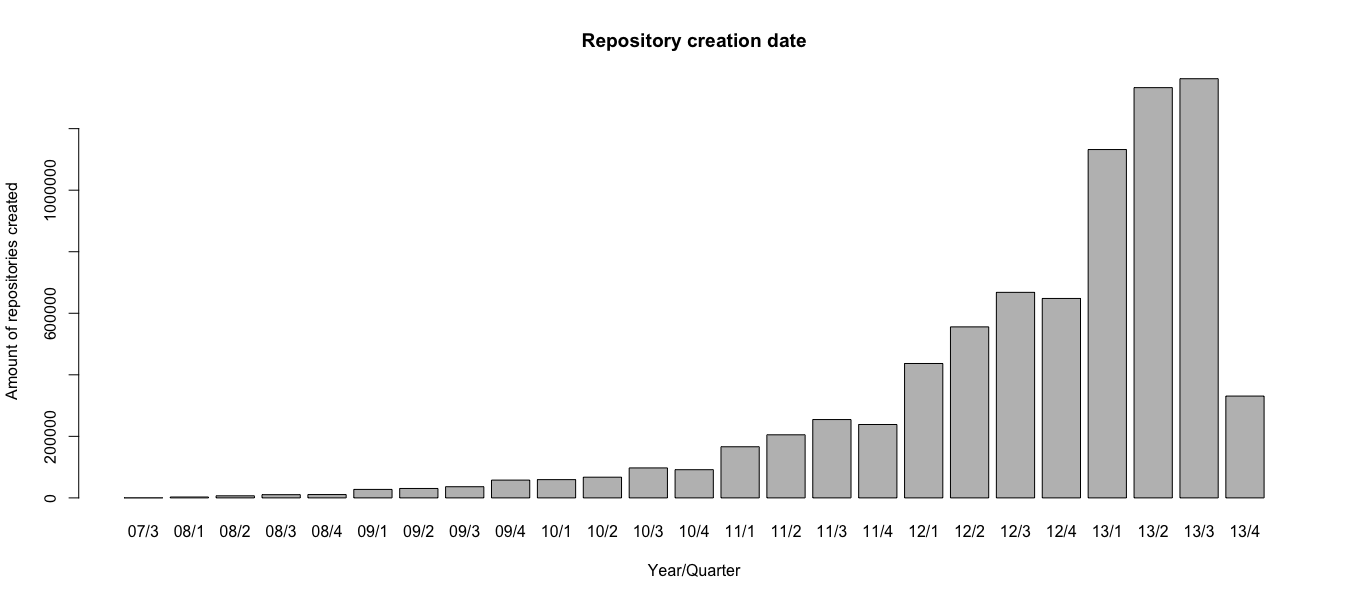
\includegraphics[width=\textwidth]{plots/repository_creation.png}
	\caption{Erstellte Projekte pro Quartal (\texttt{p.created\_date})}
	\label{projectCreation}
\end{figure}

\begin{figure}
	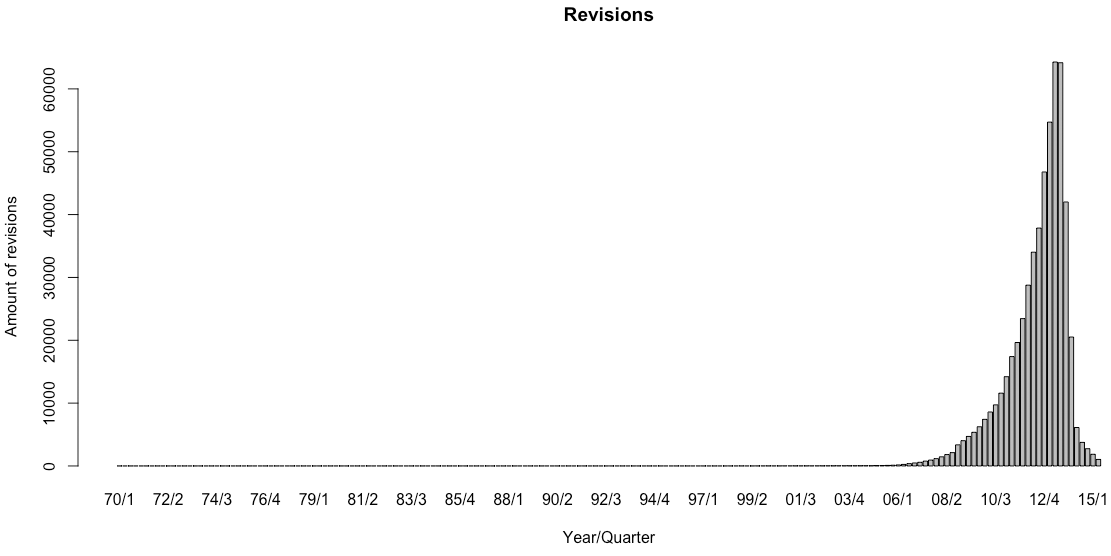
\includegraphics[width=\textwidth]{plots/revisions.png}
	\caption{Revisionen pro Quartal}
	\label{revisions}
\end{figure}


Zunächst galt es einen Betrachtungszeitraum für die Daten zu finden. Dabei fiel auf, dass es einige wenige Revisionen gab, welche zumindest laut Datensatz bereits 1970 existierten. Da diese Daten aber nur sehr gering vorhanden sind, wurde zunächst überprüft, wann die jeweiligen Projekte in dem Datensatz erstellt wurden. Hierfür wurde ein Hilfsskript entwickelt (\texttt{boa/repository\_count.boa}), welches die erstellten Projekte pro Quartal zusammenzählt (siehe Abb. \ref{projectCreation}). Als Startzeitpunkt für die Analyse der Annotationen wurde 2007/Q3 gewählt, da dort die ersten Projekte zum Datensatz hinzugefügt wurden. Frühere Revisionen werden nicht betrachtet, auch wenn diese teilweise vorhanden sind. Abbildung \ref{revisions} zeigt die Anzahl der Revisionen im zeitlichen Verlauf. Dort ist ebenfalls zu erkennen, dass die Anzahl der Projekte (und somit die Anzahl der Revisionen) ab 2007/Q3 ansteigt. Zu beachten ist, dass nur Annotationen betrachtet werden, welche in mindestens zwei Projekten verwendet werden, um auszuschließen, dass diese nur eine projektinterne Verwendung haben.\par

Auffällig ist, dass nach 2013/Q4 keine neuen Projekte mehr zum Datensatz hinzugefügt wurden. Fraglich bleibt, ob dies durch das BOA-Team entschieden wurde oder, ob die Einführung von Java 8 damit zusammenhängt, wobei das offizielle Releasedatum erst der 18.03.2014 war.

\subsection{Top 10 Annotationen}

Anschließend wurden aus dem Datensatz die Top 10 Annotationen herausgesucht. Dabei wurden zwei Kriterien beachtet. Zum einen wurden die Top 10 Annotationen im Bezug auf die Häufigkeit der Benutzung im Quellcode (Abb. \ref{top10_use}) betrachtet und zum anderen die Häufigkeit der Benutzung in verschiedenen Projekten (Abb. \ref{top10_projects}). Die \texttt{@Override} Annotation liegt dabei in beiden Varianten mit großem Abstand an der Spitze. Weiter fällt beispielsweise auf, dass die Annotation \texttt{@SuppressWarnings} zwar
in mehr Projekten verwendet wird als \texttt{@Test}, jedoch wird \texttt{@Test} insgesamt häufiger im Quellcode verwendet. Dies liegt wahrscheinlich daran, dass \texttt{@SuppressWarnings} zum Umgehen von Warnungen des Compilers verwendet wird, was bei der Entwicklung von Software ohne zusätzliche eigene Entwicklung auftreten kann, wohingegen \texttt{@Test} Unit-Testmethoden kennzeichnet, welche vom Entwickler selbst geschrieben werden müssen. Da beim Testen in der Regel mehr als ein Testfall angelegt wird, ließe dies die größere Verwendung von  \texttt{@Test} bei der Benutzung in Quellcodes gegenüber \texttt{@SuppressWarnings} erklären. Außerdem ist auffällig, dass die \texttt{@Test}-Annotation bei der Benutzung im Quellcode direkt von zwei weiteren JUnit-Test Annotationen gefolgt wird: \texttt{@TestTargetNew} und \texttt{@TestInfo}. Es ist naheliegend, dass durch die Verwendung von JUnit-Tests die Annotationen welche mit dieses Tests in Verbindung stehen häufiger verwendet werden. Ähnlich sieht es mit den Annotationen \texttt{@XmlAttribute} und \texttt{@XmlElement} aus, welche zur Verarbeitung von XML-Daten eingesetzt werden \cite{xml}.

\begin{figure}[H]
	\centering
	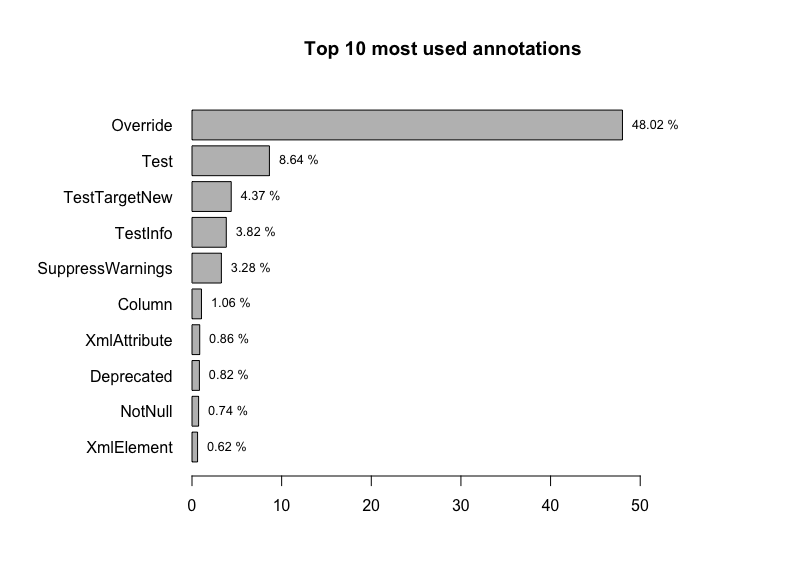
\includegraphics[width=0.8\textwidth]{plots/top10_use.png}
	\caption{Top 10 Annotationen nach Benutzung im Quellcode}
	\label{top10_use}
\end{figure}
\begin{figure}[H]
	\centering
	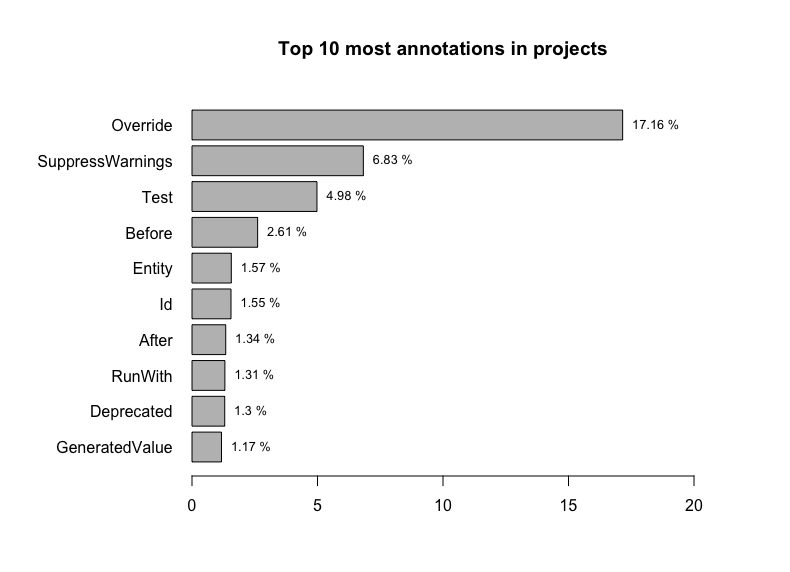
\includegraphics[width=0.8\textwidth]{plots/top10_projects.png}
	\caption{Top 10 Annotationen nach Vorkommen in verschiedenen Projekten}
	\label{top10_projects}
\end{figure}

\subsection{Annotationen im zeitlichen Verlauf}

\begin{figure}[H]
	\centering
	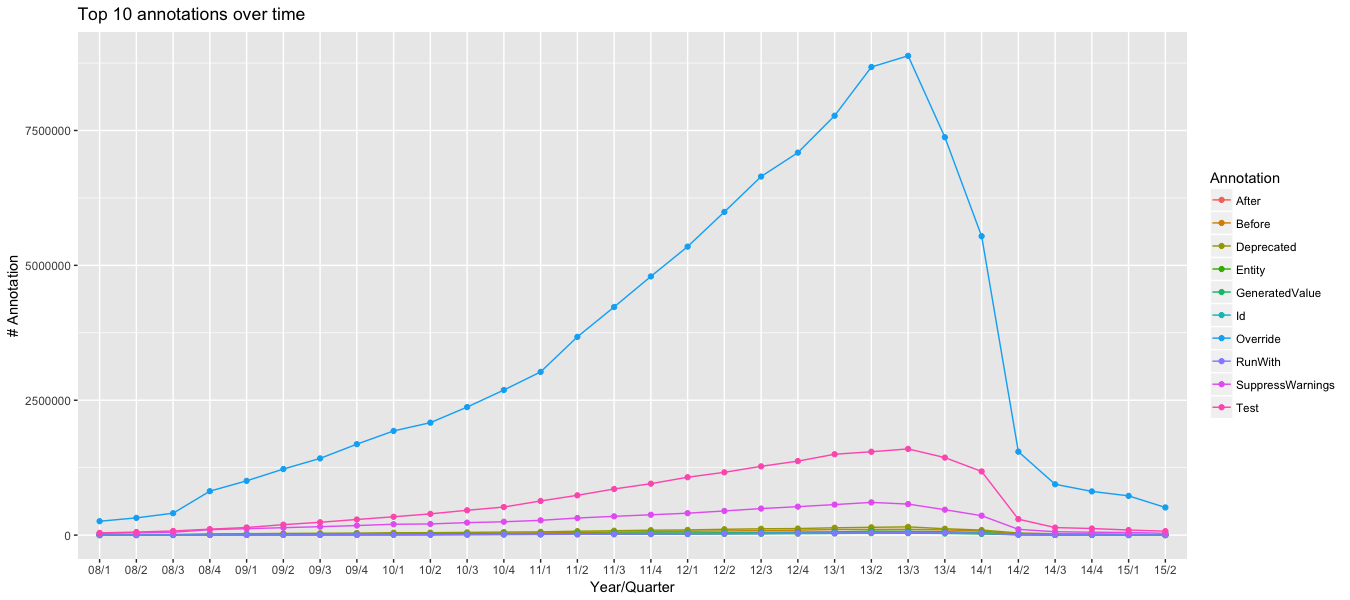
\includegraphics[width=\textwidth]{plots/absolute_top10_over_time.png}
	\caption{Top 10 Annotationen im zeitlichen Verlauf}
	\label{top10_over_time}
\end{figure}
\begin{figure}[H]
	\centering
	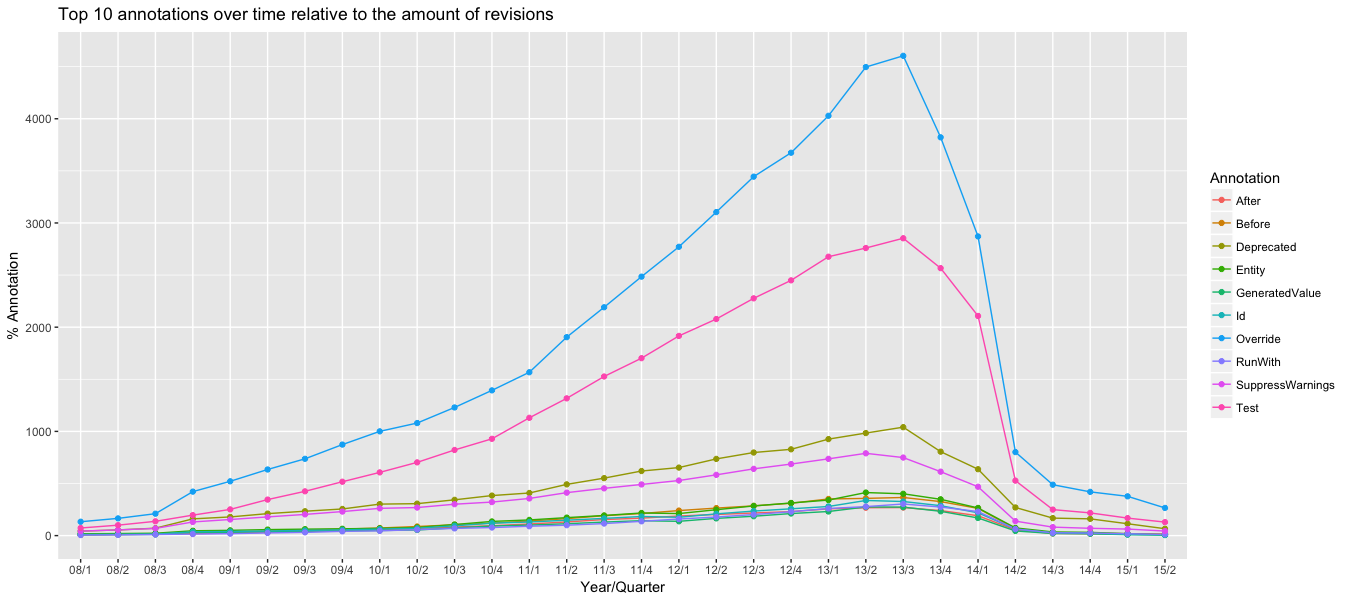
\includegraphics[width=\textwidth]{plots/top10_relative.png}
	\caption{Top 10 Annotationen im zeitlichen Verlauf - relativ zu der Anzahl an Revisionen}
	\label{top10_over_time_relative}
\end{figure}

Nachdem die Top 10 Annotationen bekannt sind, werden diese im Folgenden im zeitlichen Verlauf betrachtet. Hierfür werden die Top 10 Annotationen nach Vorkommen in Projekten verwendet (Abb. \ref{top10_projects}). In Abbildung \ref{top10_over_time} ist die zeitliche Entwicklung der Annotationen  abgebildet. Da es sich hierbei um absolute Werte handelt steigen diese bei allen Annotationen im Zeitraum zwischen 2007/Q3 und 2013/Q3 stetig an. Dies ist auf die steigende Anzahl an Projekten zurückzuführen. Auch wenn die Annotation \texttt{@Override} klar dominiert, so weisen alle Kurven einen sehr ähnlichen Verlauf auf (siehe beispielsweise Abb. \ref{deprecated}, wo die Annotation \texttt{@Deprecated} isoliert zu sehen ist). Die Anzahl der Projekte erklärt ebenfalls den extremen Abfall der Anzahl an Annotationen nach 2013/Q3, da dort keine weiteren Projekte mehr zum Datensatz hinzugefügt wurden (siehe Abb. \ref{projectCreation}) und die älteren Projekte scheinbar keine neuen Annotationen mehr hinzugefügt haben. Um die Daten etwas zu normalisieren, wurde versucht die Anzahl der Annotationen in Relation zu der Anzahl der Revisionen zu dem jeweiligen Zeitpunkt zu setzen. Dieses Ergebnis ist in Abbildung \ref{top10_over_time_relative} zu sehen. Bedauerlicherweise ist es auch in dieser Darstellung nicht möglich Rückschlüsse auf die Entwicklung einer Annotationen zu ziehen, da die Anzahl der Annotationen immer noch zu stark an die Anzahl der Projekte gebunden ist. Auch wenn die Anzahl der Annotationen in Abbildung \ref{top10_over_time_relative} relativ zu der Anzahl an Revisionen ist, so beachtet diese Darstellung nicht die Anzahl an Annotationen innerhalb der jeweiligen Revisionen, wodurch die hohen Prozentwerte von teilweise über 4000\% zustande kommen. Große Projekte mit extrem vielen Annotationen ziehen die Kurve somit immer nach oben.\par

\begin{figure}
	\centering
	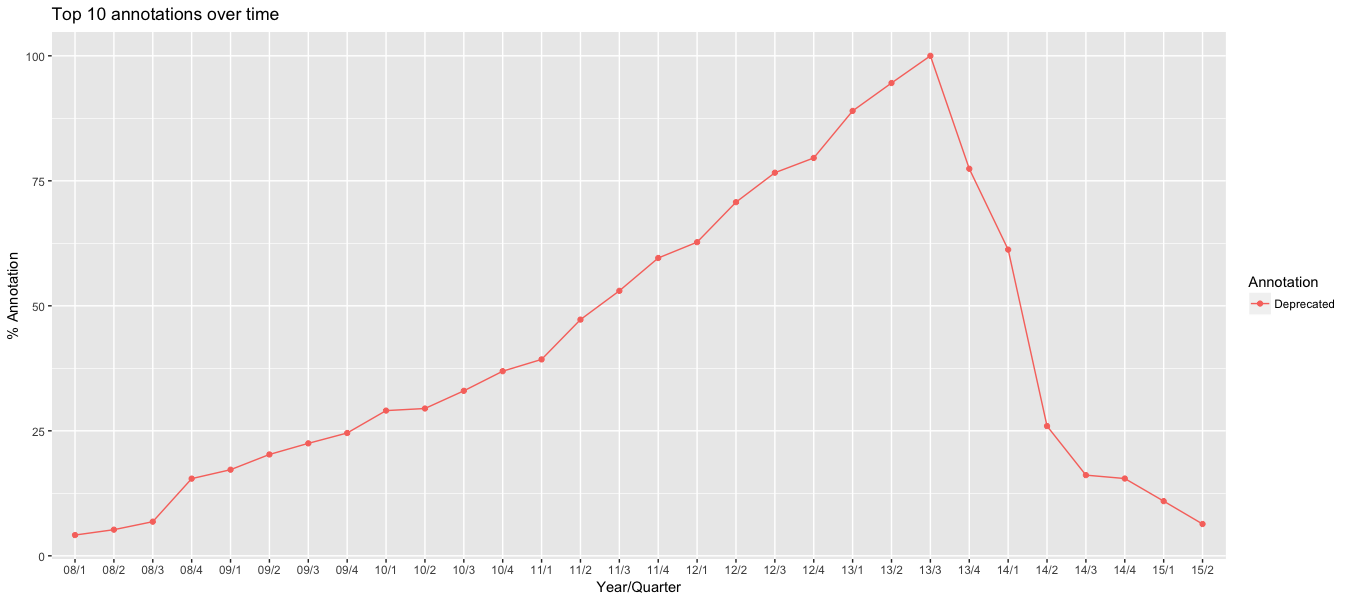
\includegraphics[width=\textwidth]{plots/deprecated.png}
	\caption{\texttt{@Deprecated} im zeitlichen Verlauf - relativ zu der Anzahl an Revisionen}
	\label{deprecated}
\end{figure}

Um dennoch die Annotationen im zeitlichen Verlauf zu betrachten, wurde das Skript zur Datenbeschaffung noch einmal etwas angepasst. In der ursprünglichen Variante wurden Projeke wie folgt betrachtet:


\begin{align*}
	& t_{start} = \text{Commit-Datum der ersten Revision + 3 Monate}\\
	& t_{end} = \text{Commit-Datum der letzen Revision + 3 Monate}
\end{align*}\\

Mithilfe einer For-Schleife wurde dann quartalsweise ein Snapshot im Zeitraum zwischen $t_{start}$ und $t_{end}$ erstellt und die Annotationen aus diesem Snapshot ausgelesen. Wenn ein Projekt allerdings nur über einen sehr kurzen Zeitraum aktiv war, wurden die Annotationen dieses Projekts ausschließlich für diesen aktiven Zeitraum gewertet und fallen danach wieder weg. Um dem entgegenzuwirken, wurde das Skript so angepasst, dass die Snapshots immer bis 2015/Q4 erstellt werden, sodass vorhandene Annotationen nicht wieder aus der Auswertung verschwinden (siehe \texttt{boa/script-modified.boa}). Leider führte dies ebenso wenig zum Erfolg. Durch diesen Versuch wurden die Kurven lediglich glatter, es ließen sich aber keine Schwankungen in der Benutzung von Annotationen feststellen (siehe Abb. \ref{top10_new}). 

\begin{figure}
	\centering
	\includegraphics[width=\textwidth]{plots/new.png}
	\caption{Top 10 Annotationen im zeitlichen Verlauf mit verändertem BOA-Skript}
	\label{top10_new}
\end{figure}


\section{Fazit}

Mithilfe von BOA und dem dort vorhandenem Datensatz war es möglich einen groben Überblick über die meistverwendeten Annotationen in Java-Projekten zu erhalten. Vor allem die Verwendung der \texttt{@Override}-Annotation fällt dabei als meistgenutzte  Annotation auf. Zusätzlich werden viele Annotationen für das Testing im Rahmen der JUnit-Tests verwendet. Das Ranking der Annotationen verändert sich auch beim Betrachten eines längeren Zeitraums nicht. Leider gaben die Daten keine Möglichkeit Schwankungen verschiedener Annotationen zu analysieren. Für zukünftige Forschungen auf diesem Gebiet sollte sich auf eine begrenzte und feste Anzahl an Repositories bezogen werden, sodass verhindert wird, dass die steigende Anzahl an Repositories die Ergebnisse beeinflusst, um so möglicherweise Veränderungen bei der Benutzung von Annotationen besser festzustellen. Es wurde versucht dies mithilfe von BOA zu realisieren, jedoch ist die Eingrenzung auf eine vordefinierte Projektmenge nicht gelungen.


\printbibliography

\end{document}